\documentclass{article}
\usepackage[utf8]{inputenc}

\title{NTIN066 - (a,b)-trees}
\author{Thuong-Hai Pham}
\date{January 2017}

\usepackage{natbib}
\usepackage{graphicx}

\begin{document}

\maketitle

\section{Uniform test}

Figure \ref{fig:uni} shows the average number of nodes accessed (avg. visits) and modified (avg. edits) in Uniform test. While `avg. visits' lines are $O(\log n)$, `avg. edits' lines are $O(1)$, as expected. (2,4)-tree lines are lower than (2,3)-tree because the higher maximum children allowed, the shorter the tree height is.

\begin{figure}[h!]
\centering
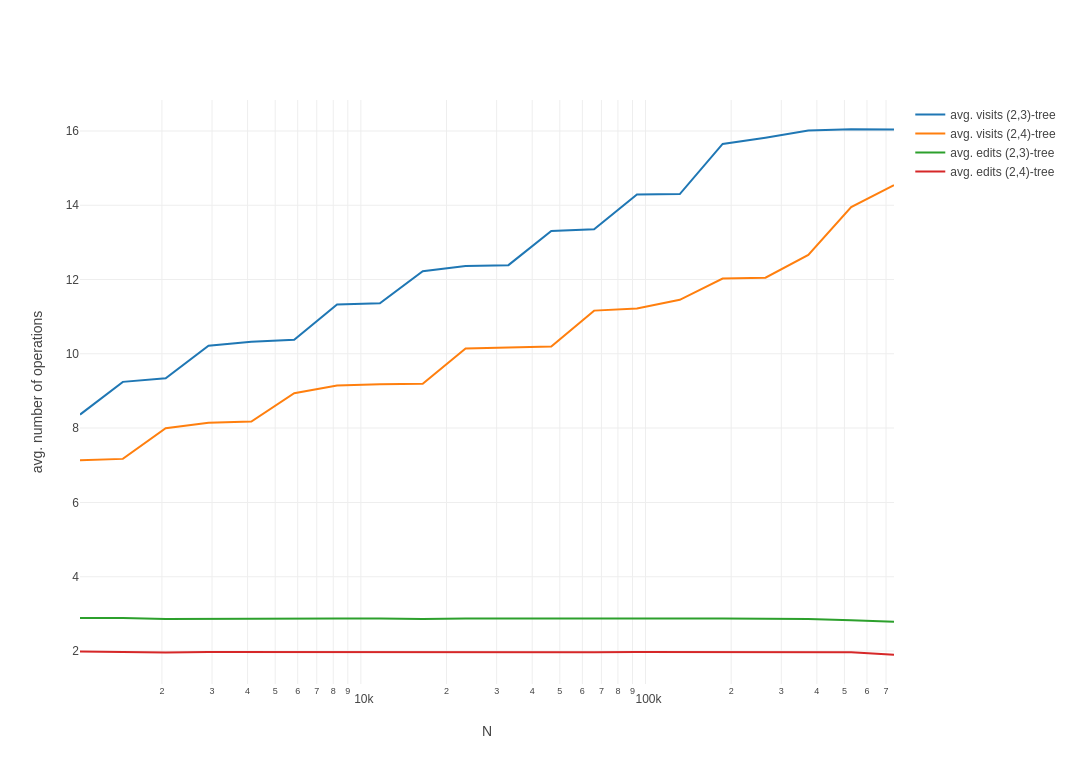
\includegraphics[width=\textwidth]{NTIN066-abtree-plot1.png}
\caption{Average number of nodes accessed (avg. visits) and modified (avg. edits) in Uniform test}
\label{fig:uni}
\end{figure}

\section{Biased test}

\begin{figure}[h!]
\centering
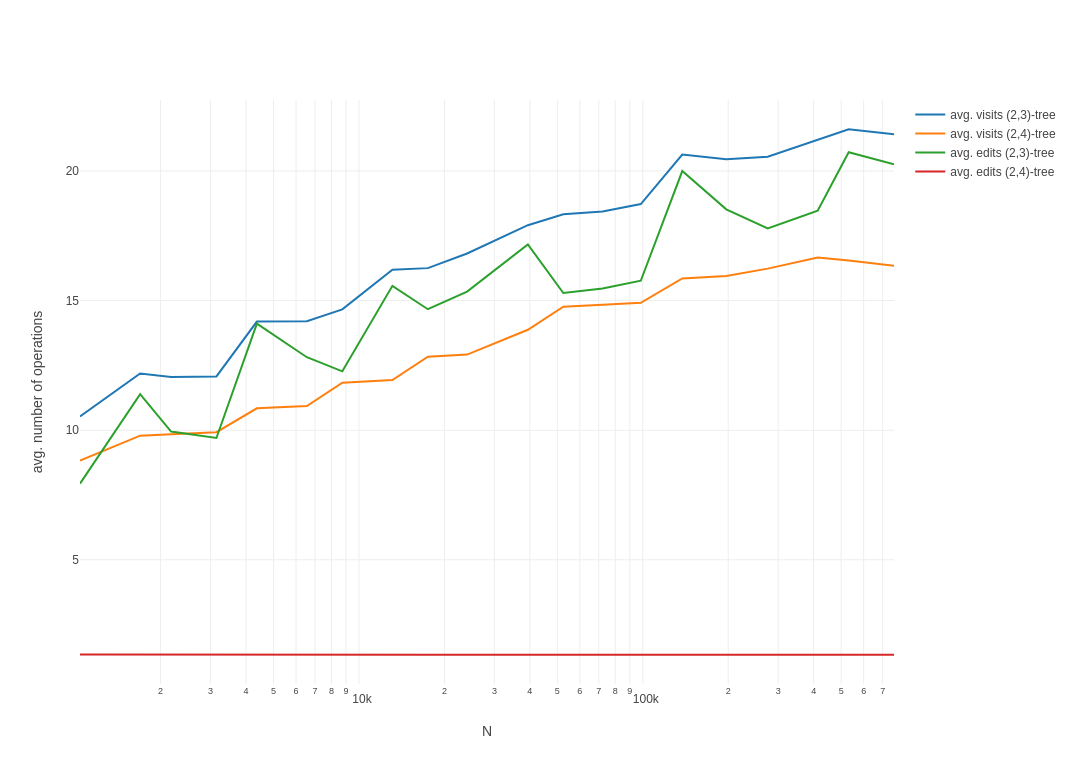
\includegraphics[width=\textwidth]{NTIN066-abtree-plot2.png}
\caption{Average number of nodes accessed (avg. visits) and modified (avg. edits) in Biased test}
\label{fig:bia}
\end{figure}

In Biased test, Figure \ref{fig:bia} shows that `avg. visits' lines are still $O(\log n)$. However, the average number of nodes modified between (2,3)-tree and (2,4)-tree differ. This difference was intentionally created by the sequence of insertions and deletions:
\begin{enumerate}
    \item The first insertion sequence from 1 to N creates a tree with most of the nodes have one key.
    \item The first deletion sequence targets on nodes that after deleting these nodes, creates many cluster of two-key leaf nodes.
    \item Then sequences of insertion and deletion of the same subset of keys are performed.
\end{enumerate}

The difference starts after step 2. Because (2,3)-tree only allows a node of maximum 2 keys, inserting a new key to these 2-key nodes grows the tree upwards all the way to the root. Then deleting that standalone key also requires fusing nodes all the way to the root. Both lead to the complexity of $O(\log n)$. While in (2,4)-tree, the maximum number of keys is 3, hence, inserting a new key to these 2-key nodes is trivial without any splitting. Similarly, deleting one key from a 3-key node requires no fusion.


\end{document}
